% ===================================================================
\chapter{Comparison with the Baseline}
\label{ch:vskiem}

Kiem's compression ratios come from private recordings of a
single-transmitter radar with real samples; this thesis's come from a public
twelve-transmitter cascade with complex samples. Three questions cannot be
answered across that gap directly. Kiem's DRHE compresses his data by 3.25 and
this thesis's DRHE compresses ColoRadar by 3.75: are the numbers comparable?
Kiem judged LPC less promising than DRHE, while this thesis's LPC is level with
it: which is right? And is this thesis's DRHE the algorithm Kiem specified?
To answer them, Kiem's MATLAB simulation was rebuilt from his text alone and
every coder of this thesis was run on it. The hardware side of the comparison
is Chapter~\ref{ch:hwinterpret}.

% -------------------------------------------------------------------
\section{Rebuilding Kiem's simulation}
\label{sec:kr_built}

The replication is a separate MATLAB code base that shares no code with the
evaluation chain of Chapter~\ref{ch:evaluation}. It follows his Figure~3.1:
beat signals of his five-target scene (his Table~3.2: one transmitter, four
receivers, 1024 samples per ramp, 512 ramps, 14-bit ADC), white Gaussian noise
set to a chosen noise floor after NCI, his pre-processing and range FFT,
quantisation to FX16, every coder, and his second-stage processing and
metrics. Every lossless path is decoded and compared with its input on every
run.

\label{sec:kr_assump}
Where his text leaves a choice open, the replication makes it explicitly and
in one place. The one that matters is the FX16 scaling. Kiem's FFT core keeps
the top 16 bits of its 32-bit output word, so the full scale of the
\emph{word} maps to \num{32767}. This thesis's chain maps the spectral peak of
a full-scale \emph{sinusoid} to \num{32767} (Equation~\eqref{eq:scale}). The
two differ by exactly a factor of four, because the Hanning window halves a
sinusoid's peak and a real sinusoid splits its amplitude between positive and
negative frequencies. The replication runs both. The other choices --- target
angles, an amplitude scaling that avoids ADC clipping, the definition of
0\,dBFS, and the detector of Section~\ref{sec:refchain} --- do not affect the
compression ratio.

% -------------------------------------------------------------------
\section{What sets the ratio on Kiem's scene}
\label{sec:kr_m75}

Table~\ref{tab:kr_m75} runs the workflow at the $-75$\,dBFS noise floor of his
Table~3.2, and at $-87.9$\,dBFS, the level that a bisection finds DRHE
reproducing his 3.25.

\begin{table}[htbp]
\centering
\caption[Coders on Kiem's rebuilt scene]{Compression ratios on Kiem's rebuilt
scene with his FFT core's scaling, at his stated noise floor and at the level
where DRHE reproduces his 3.25. FX16 noise is 20.4 and 4.6\,LSB respectively.
Every lossless coder has FX16's detection metrics.}
\label{tab:kr_m75}
\small
\begin{tabular}{@{}lrrr@{}}
\toprule
Coder & $-75$\,dBFS & $-87.9$\,dBFS & Kiem (his data)\\
\midrule
DRHE, R4S4 + run-length, ideal Huffman & 2.28 & \textbf{3.25} & \textbf{3.25}\\
DRHE, $S_4$ only, ideal Huffman & 2.28 & \textbf{3.24} & \textbf{3.24}\\
DRHE, $S_4$, Kiem's fixed dictionary & 1.85 & 3.23 & 3.17 (hardware)\\
LPC, slow time (this thesis) & 2.06 & 3.38 & ---\\
LPC-Huffman, raw ADC \cite{meucci2022}, $p = 10$ & 1.32 & 1.54 & not run\\
No prediction, fixed dictionary & 2.03 & 3.26 & ---\\
\bottomrule
\end{tabular}
\end{table}

\paragraph{DRHE gives 2.28 on Kiem's own scene, not 3.25.} The scene, chain
and algorithm are his, so his 3.25 is a property of his recordings. At
$-87.9$\,dBFS the replication reproduces his pattern exactly --- 3.25 with
run-length coding, 3.24 without, almost nothing lost to the fixed dictionary
--- but that operating point was chosen to give 3.25, and it sits
\SI{17}{\decibel} below the $-70.7$\,dBFS he reports with it.

\paragraph{Prediction does almost nothing on white noise.} With no prediction
the fixed dictionary gives 2.03 and 3.26, level with DRHE and the slow-time
LPC. Noise at ramp $m-1$ says nothing about noise at ramp $m$; the ratio is set
by how many bits of noise each value carries. Figure~\ref{fig:kr_sweep} shows
this across noise floors from $-120$ to $-60$\,dBFS. Each \SI{6}{\decibel} of
noise doubles the noise in LSB and costs about one bit per value; at very low
noise the fixed dictionary's four-bit minimum caps the ratio at 3.92; the two
scalings give the same curve shifted by \SI{12}{\decibel}.

\begin{figure}[htbp]
\centering
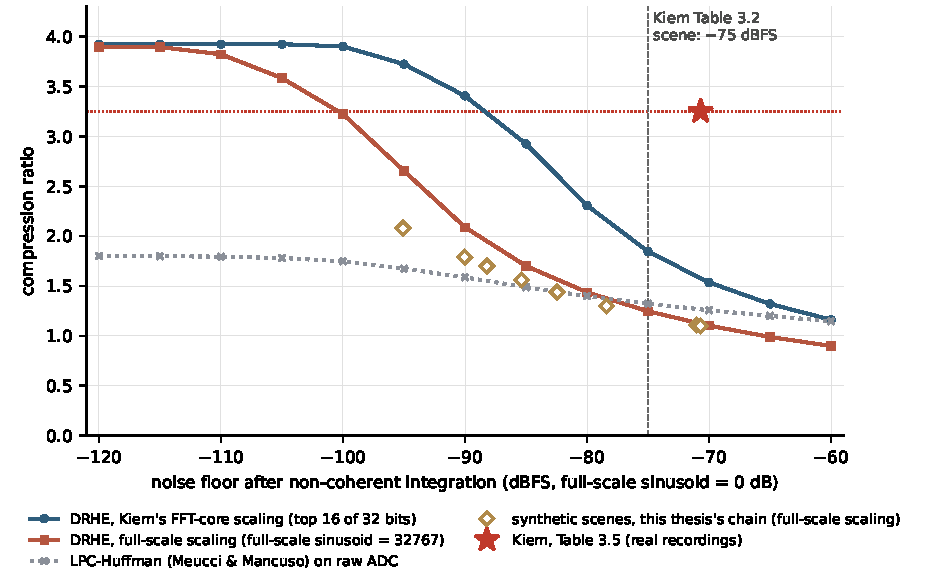
\includegraphics[width=0.85\textwidth]{fig_kr_sweep.pdf}
\caption[CR against noise floor on Kiem's scene]{Compression ratio against
noise floor on Kiem's rebuilt scene. DRHE with Kiem's fixed dictionary, with
his FFT core's scaling and with this thesis's full-scale scaling (four times
larger); LPC-Huffman of \cite{meucci2022} on raw ADC; this thesis's own chain
on synthetic scenes of the same kind; and Kiem's published 3.25 at
$-70.7$\,dBFS.}
\label{fig:kr_sweep}
\end{figure}

\paragraph{This thesis's chain gives about 1.1 on such scenes.}
\label{sec:kr_scaling}
Synthetic scenes of Kiem's kind put through this thesis's own chain, with its
full-scale scaling, compress to only 1.10--1.12 near $-70.7$\,dBFS. The
replication with the full-scale scaling gives the same 1.12 at that noise
floor, from an independent code base. Two factors multiply to explain it: the
scaling puts four times as much noise into each code (about two more bits per
value), and matching Kiem's stated noise floor with white noise puts 33\,LSB of
noise into each code even with his scaling, where his ratio needs about
4.6\,LSB. The same mechanism explains why ColoRadar compresses as well as it
does: its FX16 codes use fewer than ten of their sixteen bits
(Section~\ref{sec:decomp}).

\paragraph{His noise floor and his ratio do not agree on white noise.}
\label{sec:kr_fingerprint}
His fixed dictionary records what his residuals looked like. Coding
integer-rounded Gaussian residuals with it and with the ideal code for each
spread shows that it is optimal (overhead under \SI{0.1}{\percent}) for
residuals with a standard deviation of 6 to 8\,LSB, consistent with his ratio
and his residual histograms, and costs \SI{26}{\percent} at the 33\,LSB that
his stated noise floor implies. The most likely reconciliation is that on real
data the mean ``noisy part'' of the spectrum is raised by clutter, leakage and
sidelobes, while most cells, which set the ratio, sit much lower. That is an
inference; it cannot be confirmed without his data.

% -------------------------------------------------------------------
\section{The LPC he excluded}
\label{sec:kr_lpcraw}

LPC-Huffman as Kiem describes it predicts each raw ADC sample from the
previous $p$ samples of the same chirp, with Levinson--Durbin coefficients per
chirp and receiver sent as 32-bit floats. On his scene it loses to DRHE by a
wide margin at every order up to $p = 10$ (Table~\ref{tab:kr_m75}), and stays
below 1.8 across the whole sweep. \textbf{For the method he meant, Kiem's
ranking holds} --- but for a reason that has little to do with prediction.
His chain shifts the 14-bit samples left by 18 bits, windows them, takes the
FFT divided by $N$ and keeps the top 16 bits, so white ADC noise of standard
deviation $\sigma$ reaches the FX16 code as
\begin{equation}
\label{eq:kr_noisemap}
\sigma_{\mathrm{FX16}} = \sigma \cdot \frac{2^{18}}{2^{16}} \cdot
\frac{\sqrt{\sum_k w_k^2 / 2}}{N} = 0.0541\,\sigma,
\end{equation}
which the simulation measures exactly. The FFT scaling and truncation discard
about 4.2 bits of noise per value before DRHE sees the data; a lossless coder of
the raw samples must keep them. The truncation is the lossy step, and Kiem's
FX16 row shows its cost in detections; DRHE inherits that cost and raw-ADC LPC
does not.

The slow-time LPC of this thesis, which predicts in the same domain and along
the same axis as DRHE (Section~\ref{sec:lpc_notkiem}), is a different method,
and on the same scene it is level with or slightly ahead of DRHE: 2.06 against
1.85 and 3.38 against 3.23. On ColoRadar it is level too: 3.697 against 3.751
with Kiem's dictionary, and 4.404 against 4.218 once each has a dictionary
fitted to its own errors (Section~\ref{sec:dictresult}). The two algorithms are
within a few per cent on ratio; what separates them is that DRHE streams and
LPC needs the whole frame.

% -------------------------------------------------------------------
\section{Adding transmitters}
\label{sec:kr_tdm}

The replication can also interleave the ramps over twelve transmitters, as in
the ColoRadar cascade. On Kiem's five-target scene the transmitters make almost
no difference, because there is nothing but noise to predict. On a denser
scene of 300 slowly moving scatterers at $-95$\,dBFS --- a stand-in for a real
scene, not Kiem's --- prediction earns its keep: DRHE gives 3.40 against 1.95
without prediction on one transmitter. Interleaving twelve transmitters cuts
it to 2.37 at lag 1, and predicting from the same transmitter (lag 12)
recovers part of the loss, to 2.56. On ColoRadar, whose scene changes slowly,
the same change of lag turns a \SI{4.9}{\percent} loss against no prediction
into a \SI{7.8}{\percent} gain (Section~\ref{sec:predaxisres}).

% -------------------------------------------------------------------
\section{The DRHE algorithm, line by line}
\label{sec:kc_audit}

Table~\ref{tab:kc_audit} compares every element of Kiem's final DRHE with this
thesis's MATLAB model and HLS design.

\begin{table}[htbp]
\centering
\caption[DRHE audit against Kiem's specification]{Every element of Kiem's
final DRHE scheme (his \S{}3.5.3 and \S{}4.3.4) against this thesis's MATLAB
model and HLS design.}
\label{tab:kc_audit}
\scriptsize
\renewcommand{\arraystretch}{1.2}
\setlength{\tabcolsep}{3pt}
\begin{tabular}{@{}>{\raggedright}p{0.17\textwidth}>{\raggedright}p{0.3\textwidth}>{\raggedright}p{0.13\textwidth}>{\raggedright}p{0.22\textwidth}>{\raggedright\arraybackslash}p{0.1\textwidth}@{}}
\toprule
Element & Kiem & MATLAB model & HLS design & Same?\\
\midrule
Input & FX16 range FFT, first $N/2$ bins, per RX & same & same (128-bit AXIS, 4 RX) & yes\\
Prediction & Equations~\eqref{eq:kc_mag}--\eqref{eq:kc_phase}, $\alpha = 0.6$, $\beta = 0.4$, phase wrapped once & same, at lag $L$ & same, at lag $L$ & yes; (e)\\
Back to Cartesian & rounded to integer & \texttt{round} & \texttt{roundf} & yes\\
Difference & 16-bit two's complement & \texttt{wrap\_int16} & \texttt{wrap\_int16} & yes\\
Initial state & zero & zero per frame & zero per transmitter per frame & yes; (c)\\
State update & from the input & from the input & from the reconstruction & changed; (a)\\
$S_4$ and APPEND & his Table~3.7 & same & same & yes\\
Residual $-32768$ & no code; not addressed & counted & saturated to $-32767$ & changed; (a)\\
Dictionary & fixed, his Appendix~A & same & same, bit-reversed & yes; (d)\\
Arithmetic & fixed point & double & single-precision float & changed; (b)\\
Packing & 58-bit word per channel & bit count & 512-bit accumulator & layout; (d)\\
Lag & ramp $m-1$ (one TX) & $\nTx$ & $\nTx$ & extension; (e)\\
\bottomrule
\end{tabular}
\end{table}

The equivalence is checked by output. The replication's DRHE, written from
Kiem's text without reference to this thesis's code, and this thesis's MATLAB
model at lag 1 produce identical residuals and identical bit counts on the
replicated scene (\num{18186374} bits at $-75$\,dBFS and \num{10370342} at
$-87.9$\,dBFS). The HLS design reproduces the MATLAB model's bit counts on all
50 ColoRadar frames, an independent Python implementation reproduces the HLS
bit counts, and the board reproduces the HLS bytes
(Section~\ref{sec:verifres}). The DRHE of this thesis is therefore Kiem's,
extended in one way and implemented differently in four:

\begin{description}[leftmargin=!,labelwidth=6mm,style=sameline,font=\normalfont\bfseries]
\item[(a)] A residual of $-32768$ has no code in his scheme; the hardware
saturates it to $-32767$, and updates its state from the reconstruction so
that the encoder and decoder still agree afterwards (Section~\ref{sec:robust}).
Without saturation the closed loop gives exactly his output; on ColoRadar no
residual comes near $-32768$.
\item[(b)] Floating point follows his own suggestion for future work. It buys
\SI{0.07}{\percent} of ratio and costs most of the logic, every extra DSP and
twice the block RAM (Chapter~\ref{ch:hwinterpret}). It also does not remove
the need for a decoder built from the same source: a double-precision decoder
drifts on 8 of the 50 DRHE frames.
\item[(c)] Each transmitter's state is reset on its first ramp of every frame,
so every frame decodes on its own.
\item[(d)] The bits are his, in a different order: codewords are bit-reversed
because the packer is least-significant-bit first.
\item[(e)] The lag is $\nTx$; with $\nTx = 1$ it is his algorithm unchanged.
\end{description}

% -------------------------------------------------------------------
\section{Every result, compared}
\label{sec:kc_cr}

\paragraph{The compression ratios measure different things.} DRHE compresses
ColoRadar by 3.751 with Kiem's own dictionary, and his recordings by 3.25. The
algorithm is the same, but the ratios come from different mechanisms. On
ColoRadar, unused container bits give a factor of 1.64, the sparsity of the
range-FFT frame a further 2.12 through the entropy coder, and prediction at
lag $\nTx$ adds \SI{7.8}{\percent} (Section~\ref{sec:decomp}); at lag 1 the
same predictor \emph{costs} \SI{4.9}{\percent}. Kiem's 3.25 is what a matched
coder gives on residuals of 6 to 8\,LSB. The two chains also differ in FX16
scaling, ADC width and gain, real against complex samples, and one against
twelve transmitters, each of which moves the ratio on its own. The comparison
of \emph{algorithms} is settled by the audit; the comparison of
\emph{datasets} cannot be made, and neither the similarity of 3.25 and 3.75
nor their difference says anything about the algorithms.

\paragraph{Run-length coding adds little on both datasets.} On ColoRadar, with
ideal dictionaries, it gains at most \SI{1.6}{\percent}, because fewer than a
fifth of the residuals are zero even at lag $\nTx$. His simplification holds.

\paragraph{A fixed dictionary costs little only on the data it was fixed on.}
On his scene at $-87.9$\,dBFS his dictionary costs \SI{0.3}{\percent}. On
ColoRadar, a dictionary re-derived from frames 0--4 gains \SI{12}{\percent}
(DRHE) and \SI{18}{\percent} (LPC) on the held-out frames 5--49, because
ColoRadar's lag-$\nTx$ residuals are much smaller than the ones his dictionary
was built for.

\paragraph{Detection metrics and noise floors are not comparable.} His FX16 row
loses \SI{0.59}{\percent} of detections; this thesis's loses \SI{3.77}{\percent}
(Table~\ref{tab:stage1}). Both measure the cost of quantising to 16-bit fixed
point, but on different sensors, scenes and chains. ColoRadar's codes use 9.77
of 16 bits, so the quantisation step is coarse relative to weak returns, and
its detector integrates over transmitter-interleaved ramps. His noise floor of
$-70.7$\,dBFS and this thesis's $-105.4$\,dBFS do not share a definition of
0\,dBFS.

\begin{keybox}
\textbf{Same:} the DRHE algorithm, to the bit; that run-length coding adds
almost nothing; that DRHE beats every lossy scheme on ratio and detection
together; that the datapath meets \SI{100}{\mega\hertz} on his speed grade and
fits his device.

\textbf{Different, and explained:} every hardware resource figure, the
initiation interval and the throughput (Chapter~\ref{ch:hwinterpret}); the
value of his fixed dictionary on other data; the LPC ranking, which holds for
his LPC and not for this thesis's.

\textbf{Extended:} the prediction lag, which is $\nTx$ on a TDM-MIMO cascade;
a decompressor for every design; and verification of the hardware against
simulation byte for byte.

\textbf{Not comparable:} the compression ratios and detection metrics on the
two datasets.

\textbf{Unexplained:} his published LUT and flip-flop counts exceed what his
described design needs, and his reported noise floor is \SI{17}{\decibel}
higher than a white-noise scene with his ratio would have.
\end{keybox}
\label{ch:vskiem:end}
